% standard
\documentclass[a4paper,12pt]{article}
\usepackage[utf8]{inputenc}
\usepackage[ngerman]{babel}

% geometry
\usepackage{geometry}
\geometry{ headsep=20pt,
headheight=20pt,
left=21mm,
top=15mm,
right=21mm,
bottom=15mm,
footskip=20pt,
includeheadfoot}

% header and footer
\usepackage{datetime}
\newdateformat{dmy}{%
\THEDAY.~\monthname[\THEMONTH] \THEYEAR}
\usepackage{fancyhdr}
\pagestyle{fancy}
\lhead{Noah Vogt \& Simon Hammer}
\chead{}
\rhead{\dmy\today}
\lfoot{}
\cfoot{Gymnasium Kirschgarten}
\rfoot{Seite \thepage}
\renewcommand{\footrulewidth}{.4pt}

%for the circuit
\usepackage[siunitx, european]{circuitikz}

% fix figure positioning
\usepackage{float}

% larger inner table margin
\renewcommand{\arraystretch}{1.4}

% no paragraph indent
\setlength{\parindent}{0em}

% graphics package
\usepackage{graphicx}

\usepackage{multicol}

% use sans serif font
\usepackage{tgheros}
\usepackage{mathptmx}

% don't even ask what this is for, I have no idea (noah)
\usepackage{bm} %italic \bm{\mathit{•}}
\usepackage[hang]{footmisc}
\usepackage{siunitx}
\usepackage[font={small,it}]{caption}
\sisetup{locale = DE, per-mode = fraction, separate-uncertainty,   exponent-to-prefix, prefixes-as-symbols = false, scientific-notation=false
}
\newcommand{\ns}[4]{(\num[scientific-notation=false]{#1}\pm\num[scientific-notation=false]{#2})\cdot\num[]{e#3}\si{#4}}

% show isbn in bibliography
\usepackage{natbib}

\begin{document}

\begin{titlepage}

\vspace*{1cm}
	\centering
	
	{\scshape\Large Protokolle Praktikum Physik 3cg \par}
	\vspace{0.5cm}
	{\huge\bfseries Die experimentelle Prüfung der Kirchhoff'schen Gesetze\par}
	\vspace{0.5cm}
	{\Large Noah Vogt \& Simon Hammer\par}
	\vspace{17cm}

	{\large Durchgeführt am 26.Januar 2021\par}
	
\end{titlepage}

\tableofcontents
\pagebreak

\section{Versuchsziel}
Die Kirchhoff'sche Gesetze sollen mittels eines Experiments überprüft werden. Dazu wurde ein Schaltkreis vorgegeben, der auf einem Steckbrett nachkonstruiert werden sollte. Mit einer Messung von Spannung und Stromstärke an spezifischen Stellen der Schaltung und Berechnung der Schaltung sollten die oben erwähnten Gesetzmässigkeiten überprüft und bestätigt werden.\\

Wenn nämlich die Rechnung und gemessenen Werte - im Rahmen einem gewissen zu erwartenden Fehlerbereich - übereinstimmen, sind die Gesetze experimentell bestätigt.
\section{Physikalischer Hintergrund}

\subsection{Kirchhoffischen Gesetze}
\subsubsection{Maschenregel}

Wird ein geschlossener Teilstromkreis ("Masche") betrachtet so gilt, dass die Summe der 
Teilspannungen der der Totalspannung entspricht. Liegt an der Masche kein Spannungsquelle an so
gilt:

\[\sum_{k = 1}^{n} I_k = 0 \]
%\[ \sum_{n=0}^N


\subsubsection{Knotenregel}

Die Summe der eingehenden Ströme ist gleich der Summe der ausgehend Ströme in jedem 
Verzweigungspunkt ("Knoten"):

\[\sum I_{ein} = \sum I_{aus}\]


\subsection{Serieschaltung}

\begin{figure}[H]

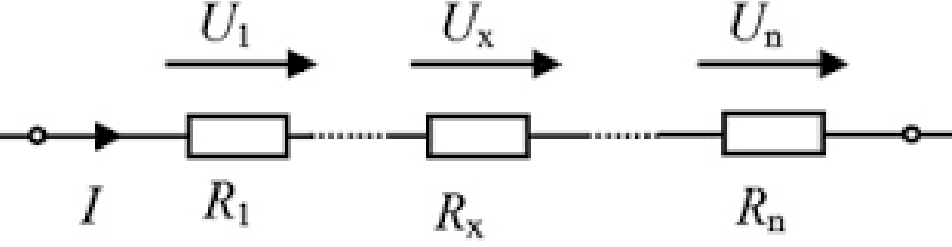
\includegraphics[width=.4\textwidth]{media/SerieschaltFert.png}

Die Knotenregel sagt aus, dass der selbe Strom $I_0$ durch alle Wiederstände $R_i$ fliesst. Durch
die Maschenregel ergibt sich dann:

\[U_0 = \sum_{k=1}^{n} R_k I_0 ,\ I_0 = \frac{U_0}{\sum_{k=1}^{n} R_k }\] 

Die Spannung teilt sich somit direkt proportional auf die einlenen Wiederstände auf.

\end{figure}

\newpage

\subsection{Parallelschaltung}

\begin{figure}[H]

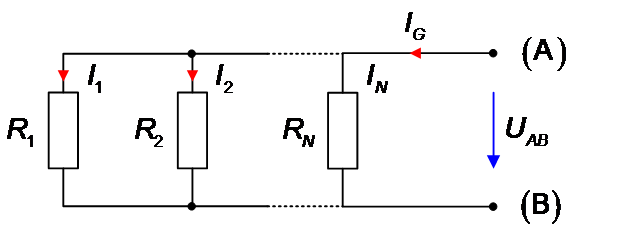
\includegraphics[width=.4\textwidth]{media/ParallelschaltungFert.png}

\end{figure}

Nach der Maschenregel liegt über allen Wiederständen die gleiche Spannung $U_0$ und nach der 
Knotenregel beträgt die Summe der Teilströme den Gesamtstrom $I_0$:

\[ I_0 = \sum_{k=1}^{n} I_k \]

und 

\[ U_0 = R_1 I_1 = R_2 I_2 = ...R_n I_n \]

Der Strom wird also indirekt Proportional zu den Wiederständen aufgeteilt. \\
Nach Auflösen der zweiten Gleichung nach $I_j$ mit $1 \leq j \leq n$ und einsetzen in die erste
ergibt sich:

\[ I_0 = \frac{U_0}{R_1} + \frac{U_0}{R_2} + ... + \frac{U_0}{R_n} = U_0 \sum_{n=1}^k \frac{1}{R_n} \]



\subsection{Ersatzwiederstand}

Die Gesamtstromstärke $I_0$, ist die Stromstärke, welche vor dem ersten Knoten herscht. \\
Die Gesamtspannung $U_0$, ist die Spannung, welche an das Stromnetz angelegt wird. \\
Wird das ganze Wiederstandsnetz mit einem Wiederstand ersetzt, so heisst dieser Ersatzwiederstand. 

\[ R_E = \frac{U_0}{I_0} \]

Der Ersatzwiederstand verändert \textit{nicht} die Gesamtstromstärke. 

\section{Versuchsaufbau}
%\begin{figure}[H]

%\centering
%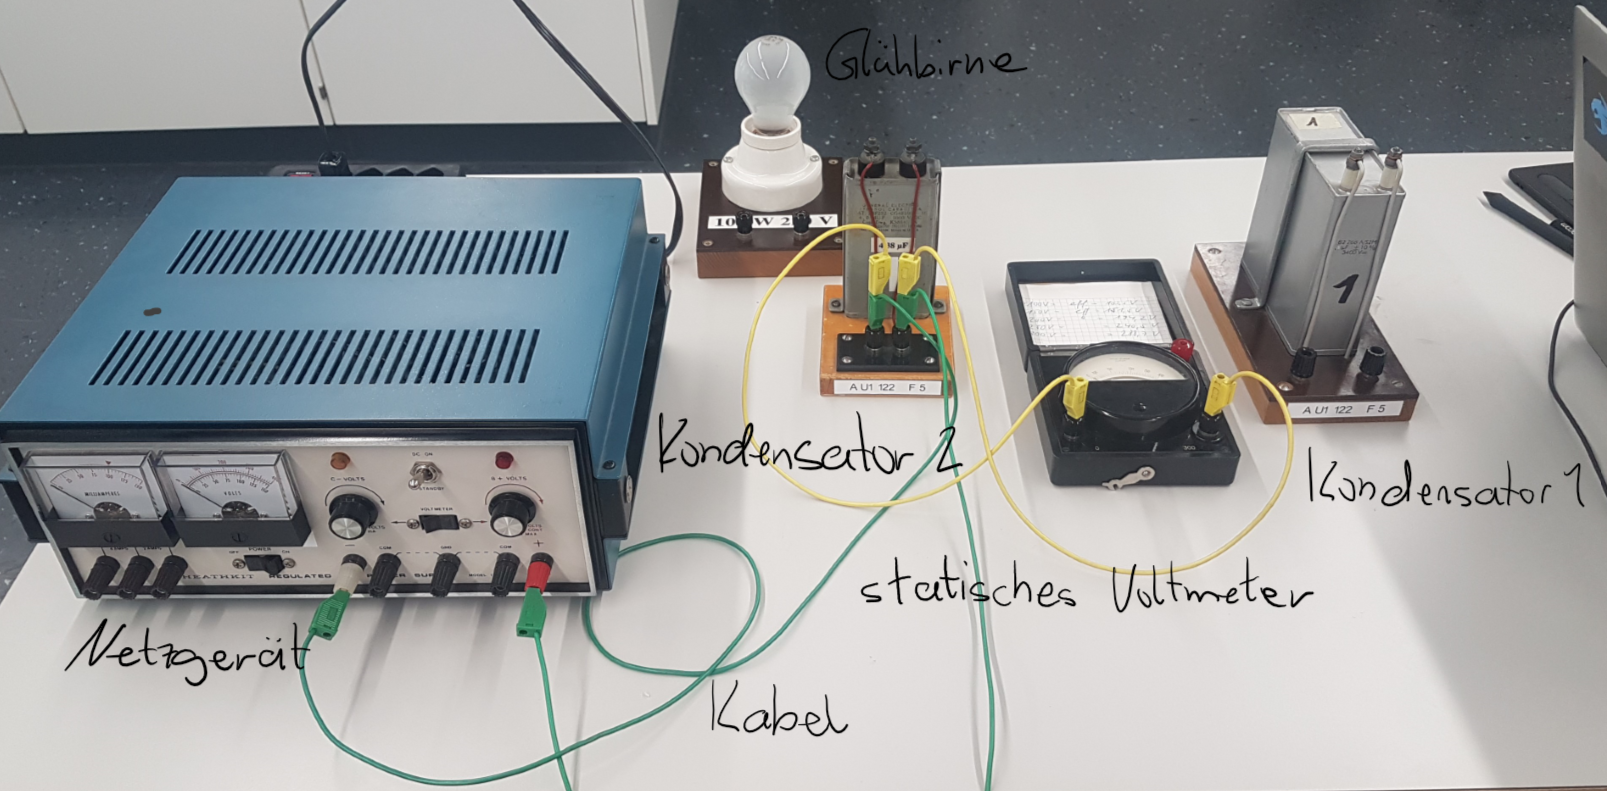
\includegraphics[width=.8\textwidth]{media/bennenung.png}

\rotatebox[origin=c]{90}{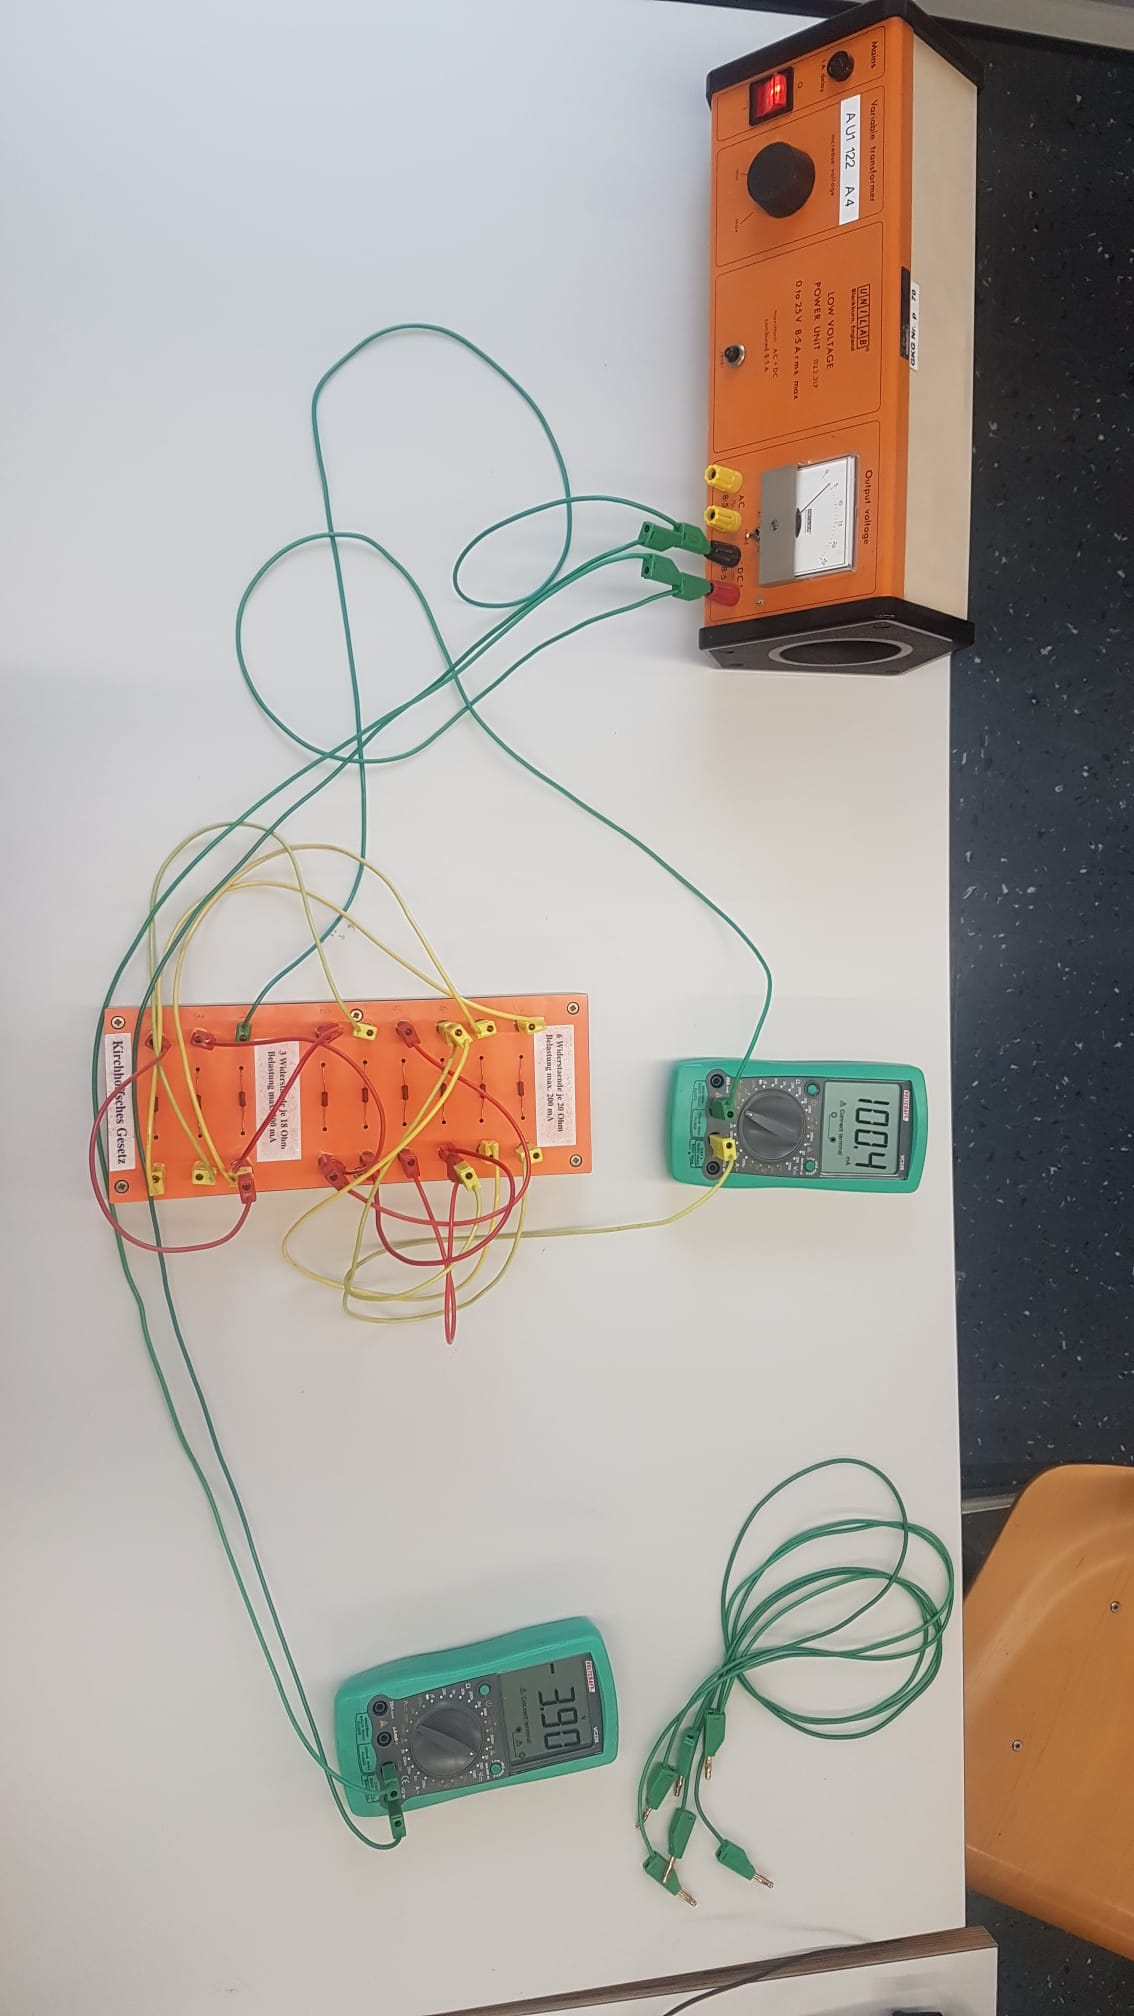
\includegraphics[width=.5\textwidth]{media/ExpSchaltQuerAll.jpeg}}


\begin{center}
\begin{circuitikz}[scale = 2.2]

    %circuit
    \draw (0,0) 
        to[isource, l=$I_0$, i=$I_0$] (4,0) 
        to [R=$R_1$ (\SI{18}{\ohm}), -*] (4,2)
        to [R=$R_2$ (\SI{20}{\ohm}), -*] (3,2)
        to [short]     (3,1.5)
        to [R=$R_3$ (\SI{18}{\ohm})]     (2,1.5)
        to [R=$R_4$ (\SI{20}{\ohm})]     (1,1.5)
        to [short, -*] (1,2)
        to [short, -*] (0,2)        
        to[ammeter, l=$A$] (0,0) --  (0,0);

    \draw (1,2)
        to [short] (1,2.5)
        to [R=$R_5 $(\SI{20}{\ohm})] (3,2.5) 
        to [short] (3,2);
    
    \draw (0,2)
        to [R=$R_6$ (\SI{20}{\ohm})]     (0,4)
        to [short, -*] (1,4)
        to [short]     (1,3.5)
        to [R=$R_7$ (\SI{20}{\ohm})]     (3,3.5)
        to [short, -*] (3,4)
        to [short]     (4,4)
        to [short]     (4,2);

    \draw (1,4)
        to [short]      (1,4.5)
        to [R=$R_9$ (\SI{20}{\ohm})]      (2,4.5)
        to [R=$R_8$ (\SI{18}{\ohm})]      (3,4.5)
        to [short]      (3,4);

    %arrows
    \draw (3.85,2)node[flowarrow,color = red, rotate = 180, label = \color{black}$I_1$]{};
    \draw (3,2.13)node[flowarrow,color = red, rotate = 90, label = left: \color{black}$I_3$]{};
    \draw (3,1.8)node[flowarrow,color = red, rotate = -90, label = left: \color{black}$I_4$]{};
    \draw (0.85,2)node[flowarrow,color = red, rotate = 180, label = \color{black}$I_1$]{};
    \draw (4,2.13)node[flowarrow,color = red, rotate = 90, label = right: \color{black}$I_2$]{};
    \draw (3,4.13)node[flowarrow,color = red, rotate = 90, label = left: \color{black}$I_5$]{};
    \draw (3,3.8)node[flowarrow,color = red, rotate = -90, label = left: \color{black}$I_6$]{};
    \draw (0.85,4)node[flowarrow,color = red, rotate = 180, label = \color{black}$I_2$]{};
    \draw (0,1.8)node[flowarrow,color = red, rotate = -90, label = left: \color{black}$I_0$]{};






\end{circuitikz}
\end{center}

\section{Versuchsdurchführung}


Zuerst wurde das ganze Steckbrett mit den integrierten Widerständen verkabelt nach Vorgabe und das Ampèremeter angeschlossen. Entsprechend den herrschenden Widerständen und erwarteten maximalen Stromstärken und Spannungen mussten die Einstellungen an Volt- und Ampèremeter angepasst werden. Nach genauem Nachkontrollieren, ob das Steckbrett wirklich korrekt aufgebaut worden ist, wurde schliesslich das Netzgerät an die Schaltung angeschlossen. \\

Dann wurde die Spannung am Netzgerät erhöht, sodass die Funktionalität der Widerstände sich zeigen konnte. Das Voltmeter wurde für die Messungen einzeln zu jedem Wiederstand parallelgeschalten und der angezeigte Wert wurde abgelesen. Mit einer Achtung darauf, ob eines der Kabel, Messgeräte oder Wiederstände durchbrennen, wurde das Netzgerät noch wenige Minuten angelassen. Es wurde aber auch darauf geachtet, dass sich kein Wasser in der Nähe des Versuchesaufbaues befand und die Spannung am Netzgerät nur konservativ erhöht wurde, um den Fall eines durchbrennenden Widerstands vorbeugend zu minimieren.\\

Nach erfolgreichem Abschluss der Messung wurde das Netzgerät wieder abgeschalten, vom Netz getrennt und alle sonstigen am Steckbrett angeschlossenen Gerätschaften wieder entfernt und versorgt.

%Als erstes wird die Kapazität vom \textit{Kondensator 2} abgelesen und an das Netzgerät mit den Kabeln angeschlossen. Das \textit{statische Voltmeter} wird an den \textit{Kondensator 2} angeschlossen und das Netzgerät wird angeschaltet. Der \textit{Kondensator 2} wird mit einer gewissen Menge Volt geladen, welche vom \textit{Voltmeter} ablesen wird. Die Kabel werden von dem Netzgerät entfernt - ohne eine Berührung mit etwas anderem - und in den \textit{Kondensator 1} gesteckt. Die Spannung wird nach dieser Parallelschaltung der beiden Kondensatoren nochmals gemessen, wenn diese stabil ist. Nun werden die Kondensatoren einzeln mit der Glühbirne Parallelgeschalten und dadurch entladen. Der ganze Vorgang wird schliesslich dreimal wiederholt mit unterschiedlicher Ausgangsspannung. 

\newpage

\section{Versuchsauswertung}

\subsection{Ersatzwiderstände berechnen}

Um die obere Masche mit den Widerständen $R_7$, $R_8$ und $R_9$ (siehe Schaltkreis in 3.) zu vereinfachen, beginnen zuerst mit der Vereinfachung der Serieschaltung.

$$R_{8,9} = R_9 + R_8 = 20 \Omega + 18 \Omega = 38 \Omega$$

Dann folgt die Parallelschaltung.

$$R_{7,8,9} = \frac{R_{8,9} \cdot R_7}{R_{8,9} + R_7} = \frac{38 \Omega \cdot 20 \Omega}{38 \Omega + 20 \Omega} = \frac{380}{29}\Omega$$\\

Analog dazu lässt sich der obere Rechenweg auch anwenden auf die untere Masche mit $R_3$, $R_4$ und $R_5$.

$$R_{3,4} = R_4 + R_3 = 20 \Omega + 18 \Omega = 38 \Omega$$

$$R_{3,4,5} = \frac{R_{3,4} \cdot R_5}{R_{3,4} + R_5} = \frac{38 \Omega \cdot 20 \Omega}{38 \Omega + 20 \Omega} = \frac{380}{29}\Omega$$\\

Nun vereinfachen wir die entstandenen Serieschaltungen von jeweils $R_{3,4,5}$ mit $R_2$ und $R_{7,8,9}$ mit $R_6$.

$$R_{6,7,8,9} = R_6 + R_{7,8,9} = 20 \Omega + \frac{380}{29} \Omega = \frac{960}{29} \Omega$$

$$R_{2,3,4,5} = R_2 + R_{3,4,5} = 20 \Omega + \frac{380}{29} \Omega = \frac{960}{29} \Omega$$\\

Nun können $R_{2,3,4,5}$ und $R_{6,7,8,9}$ parallelgeschaltet werden.

$$R_{2,3,4,5,6,7,8,9} = \frac{R_{2,3,4,5} \cdot R_{6,7,8,9}}{R_{2,3,4,5} + R_{6,7,8,9}} = \frac{\frac{960}{29}\Omega \cdot \frac{960}{29}\Omega}{\frac{960}{29}\Omega + \frac{960}{29}\Omega} = \frac{480}{29}\Omega$$\\

Mit einer letzten Serieschaltung mit $R_1$ gelangen wir zum gesamten Ersatzwiderstand $R_{ges}$.

$$R_{ges} = R_{2,3,4,5,6,7,8,9} + R_1 = \frac{480}{29}\Omega + 18\Omega = \frac{1002}{29}\Omega = 34.55\Omega$$

\subsection{Stromspannungen berechnen}

\subsubsection{Gesamtstromstärke $I_{ges}$}

\subsubsection{Teilstromstärken $I_{1\;,\;2\;,\; ...\;,\; 9}$}

%$$C_u = \frac{C_b \cdot u - u' \cdot C_b}{u'}$$

%$C_{u_{max}} = \displaystyle{\frac{C_{b_{max}}\cdot u_{1_{max}}-u_{1_{min}}'\cdot C_{b_{min}}}{u_{1_{min}}'}}$\\\\
%
%$C_{u_{max}} = \displaystyle{\frac{4.385\cdot 10^{-6}\;F\cdot 262.5\;V-175.5\;V\cdot 4.375\cdot 10^{-6}\;F}{175.5\;V}} = 2.184\cdot 10^{-6}\;F$\\\\
%
%$C_{u_{min}} = \displaystyle{\frac{C_{b_{min}}\cdot u_{1_{min}}-u_{1_{max}}'\cdot C_{b_{max}}}{u_{1_{max}}'}}$\\\\
%
%$C_{u_{min}} = \displaystyle{\frac{4.375\cdot 10^{-6}\;F\cdot 257.5\;V-180.5\;V\cdot 4.385\cdot 10^{-6}\;F}{180.5\;V}} = 1.856\cdot 10^{-6}\;F$\\\\
%
%$\Rightarrow C_{u_1}=\displaystyle{\frac{C_{u_{max}}+C_{u_{min}}}{2}} = 2020052 (\pm 163709)\cdot F = 2.02 (\pm 0.16)\; \mu F$
%
%\subsection{Durchführung 2}
%
%$C_{u_{max}} = \displaystyle{\frac{C_{b_{max}}\cdot u_{2_{max}}-u_{2_{min}}'\cdot C_{b_{min}}}{u_{2_{min}}'}}$\\\\
%
%$C_{u_{max}} = \displaystyle{\frac{4.385\cdot 10^{-6}\;F\cdot 302.5\;V-198.5\;V\cdot 4.375\cdot 10^{-6}\;F}{195.5\;V}} = 2.343\cdot 10^{-6}\;F$\\\\
%
%$C_{u_{min}} = \displaystyle{\frac{C_{b_{min}}\cdot u_{2_{min}}-u_{2_{max}}'\cdot C_{b_{max}}}{u_{2_{max}}'}}$\\\\
%
%$C_{u_{min}} = \displaystyle{\frac{4.375\cdot 10^{-6}\;F\cdot 297.5\;V-203.5\;V\cdot 4.385\cdot 10^{-6}\;F}{203.5\;V}} = 2.011\cdot 10^{-6}\; F$\\\\
%
%$\Rightarrow C_{u_2}=\displaystyle{\frac{C_{u_{max}}+C_{u_{min}}}{2}} = 2176861 (\pm 165977)\cdot F = 2.18 (\pm 0.17)\; \mu F$
%
%\newpage
%\subsection{Durchführung 3}
%
%$C_{u_{max}} = \displaystyle{\frac{C_{b_{max}}\cdot u_{3_{max}}-u_{3_{min}}'\cdot C_{b_{min}}}{u_{3_{min}}'}}$\\\\
%
%$C_{u_{max}} = \displaystyle{\frac{4.385\cdot 10^{-6}\;F\cdot 282.5\;V-189.5\;V\cdot 4.375\cdot 10^{-6}\;F}{189.5\;V}} = 2.162\cdot 10^{-6}\; F$\\\\
%
%$C_{u_{min}} = \displaystyle{\frac{C_{b_{min}}\cdot u_{3_{min}}-u_{3_{max}}'\cdot C_{b_{max}}}{u_{3_{max}}'}}$\\\\
%
%$C_{u_{min}} = \displaystyle{\frac{4.375\cdot 10^{-6}\;F\cdot 277.5\;V-194.5\;V\cdot 4.385\cdot 10^{-6}\;F}{194.5\;V}} = 1.857\cdot 10^{-6}\; F$\\\\
%
%$\Rightarrow C_{u_3}=\displaystyle{\frac{C_{u_{max}}+C_{u_{min}}}{2}} = 2009486 (\pm 152519)\cdot F = 2.01 (\pm 0.15)\;\mu F$

\section{Kommentar / Diskussion}

\subsection{Genauigkeit}

Da die Kapazität des \textit{Kondensators 1} nicht bekannt ist, kann keine genaue Aussage über die Genauigkeit des Experiments getroffen werden. Es wird aber immernoch eine Abweichung vom realen Wert angenommen, weil dieses Experiment gewisse Fehlerquellen aufweist (dazu später mehr). Ebenso wird von einer richtigen Berechnung ausgegangen.\\



%-Voltmeter recht ungenau, verbraucht vllt. sogar noch strom

%Bei der Durchführung eins und drei ist eine sehr geringe Abweichung der Endresultate zu verzeichen. Zu dem Wert von Durchführung zwei ist aber auch nur eine kleine Abweichung zu verzeichenen. Es wird somit angenommen, dass bei \textit{keinem} der drei Durchgängen ein grosser Fehler unterlaufen ist. Aber leider lässt sich durch keine Beobachtung erklären, weshalb es zu dieser Abweichung beim Endresultat der zweiten Durchführung kam.

%-energie geht verloren ein wenig bei der der parallelschaltung (keine 100\% ige effizienz)

%-(wärme geht an umwelt verloren)

%Bei den beiden Versuchsdurchgängen wurden beim ersten Mal eine Abweichung von \textit{13\%} und beim zweiten Mal \textit{37\%} festgestellt.\\

%Aufgrund der vielen systematischen Fehler, da nicht in einem abgschlossenen System experimentiert werden konnte, kann die Ungenauigkeit der Messresultate erklärt werden. Der Tabellenwert $\num{3.338 e5}\si{\J\per\kg}$ \cite{formelsammlung} wurde wie erwartet unterschritten, da einige Energie aus unserem System an die Umgebung verloren ging.\\

%Es ist noch anzumerken, dass bei der Berechnung keine Fehlerschranke bei der Masse gemacht wurde. Dies ist zu begründen, dass diese Ungenauigkeit im Vergleich zur Temperaturmessung vernachlässigbar ist.

\subsection{Fehlerquellen}

Ein Fehler besteht darin, dass das Voltmeter sehr ungenau misst und gleichzeitig wahrscheinlich auch noch ein wenig Strom verbraucht. Es wird auch angenommen, dass die Kondensatoren nicht 100\% der Ladung gespeichert halten können. Nur ist die Zeit, in welcher die Kondensatoren Energie abgeben können sehr kurz, und es wird aufgrund dessen mit einer kleinen Verfälschung des Ergebnissses gerechnet.\\

Es geht Energie verloren sobald die Kabel vom Netzgerät in den \textit{Kondensator 1} gesteckt werden, da es meist blitzt beim Ein- oder Ausstecken der Kabel. Da Licht auch Energie ist, kann abgeleitet werden, dass dort Strom verloren geht. Es wird nicht angenommen, dass diese Verfälschung des Ergebnisses gross ist.\\

Eine weitere Fehlerquelle besteht darin, dass die verwendeten Kabel wahrscheinlich nicht zu 100\% isoliert sind und somit ein kleiner Teil des übertragenen Stromes als Wärme verloren geht.


%Ein systematisch Fehler bestand darin, dass das Kalorimeter nicht zu 100\% isoliert und durch die Wände konstant Energie an die Umwelt abgegeben wird. Vorallem da das Kalorimeter nach oben offen war, entstanden dabei beträchtlich mehr Wärmeverluste am Wasser an die Umgebung als nur den Wänden.\\

%Ein weiterer Fehler bestand darin, dass das Eis nicht vollständig mit dem Papier abgetrocknet werden konnte.\\

%Beim der zweiten Versuchsdurchführung ist ein kleiner Fehler unterlaufen: Das Eis ist auf den Tisch gefallen und wurde dann mit dem Händen in das Kalorimeter befördert. Dabei ist ein Teil des Eises geschmolzen, weil Wärmeenergie von den Händen an das Eis abgegeben wurde. Somit ist die höhere Abweichung vom Tabellenwert im Vergleich zum ersten Versuchsdurchlauf begründet.

\end{document}
